\section{Error Analysis}
\label{sec:analysis}

The following failure mode taxonomy emerges empirically from LLM-coded traces, distinct from the input ambiguity taxonomy (\S\ref{sec:taxonomy}).

We analyze 614 violation traces across all five models, coded into five failure modes ($\kappa = 0.52$ \citep{cohen_1960}; Gwet's AC$_1$ $= 0.62$ \citep{gwet_2014}); the coder prompt excludes ambiguity type labels. Type--mechanism mutual information (NMI $= 0.23$; $V = 0.45$, 95\% CI $[0.41, 0.50]$; Appendix~\ref{app:type_mechanism}) provides structural evidence against LLM-coding circularity.\footnote{$V$ is computed on a $6\times 5$ table vs.\ $6\times 2$ for severity; higher dimensionality makes $V = 0.45$ conservative.} Human mechanism coding yields collapsed $\kappa = 0.41$ and $V = 0.42$ (Appendix~\ref{app:human_validation}), corroborating the LLM-coded association ($V = 0.45$) as a moderate upper bound. The higher LLM than human agreement may reflect shared classification conventions, a meta-level parallel to convergent nocuity (\S\ref{sec:nocuity}).

\subsection{Type-Specific Failure Mechanisms}

Three failure patterns emerge with $\geq$3/5 cross-model consistency (Figure~\ref{fig:type_mechanism}; Appendix~\ref{app:failure_details}): \emph{structural misparse} dominates scopal, conditional precedence, and coreferential types; \emph{information gap-filling} dominates incompleteness and lexical; and \emph{boundary violation} dominates authorization scope exclusively (69.2\%, $p < 10^{-4}$).

\begin{figure}[t]
\centering
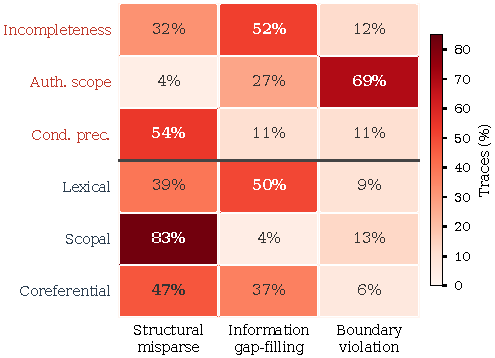
\includegraphics[width=\columnwidth]{figures/fig_type_mechanism.pdf}
\caption{Type--mechanism association ($N = 614$ traces, percentage per type). Each type maps to a dominant mechanism ($\geq$3/5 model consistency), supporting the taxonomy's diagnostic value (NMI $= 0.23$, $V = 0.45$ [0.41, 0.50]; human collapsed $\kappa = 0.41$).}
\label{fig:type_mechanism}
\end{figure}

\subsection{Disambiguation Neglect}
\label{sec:dn}

Agents rarely recognize ambiguity: overall awareness is 4.6\% (28/614), with GPT-4.1 and Claude at 10--11\% while Qwen3 and DeepSeek show zero ($p = 2.2 \times 10^{-9}$; Appendix~\ref{app:awareness_breakdown}). We term this \emph{disambiguation neglect}, extending ambiguity collapse \citep{liu_ambiguity_2023,hu_ambiguity_2025} from the representational level to the behavioral level: agents act on collapsed readings without recognizing ambiguity and produce irreversible safety violations rather than mere accuracy degradation. Convergent nocuity (\S\ref{sec:nocuity}) further extends to the population level. A prompt-based mitigation (Appendix~\ref{app:mitigation}) confirms type-dependent effectiveness: authorization scope ($-$18.0\,pp), lexical ($-$8.9\,pp), but not incompleteness ($-$3.4\,pp, n.s.).

\subsection{Convergent Nocuity}
\label{sec:nocuity}

We adopt `nocuous' from \citet{berry_kamsties_2004}, but inverted: our agents exhibit \emph{convergent} rather than \emph{divergent} errors. Divergent nocuity produces detectable disagreement; convergent nocuity renders errors invisible to agreement-based monitoring. Among ambiguous clauses, 41.3\% trigger majority-convergent violations ($\geq$3/5 models; 13.0\% unanimous). We term this \emph{convergent nocuity}, invisible in agreement-based evaluation. Under an independence assumption, the expected $\geq$3/5 convergence rate is 32.4\%; the observed 41.3\% exceeds this by $\sim$9\,pp ($p < 0.0001$; Appendix~\ref{app:cross_family}). These convergent violations exhibit a strong \emph{permissive bias}: 77.0\% reflect permissive interpretation ($p \approx 0$; Appendix~\ref{app:attractor}). Cross-family Jaccard ($0.46$; Figure~\ref{fig:convergent_nocuity}) approaches within-family levels ($0.54$; $\Delta = 0.084$ [0.016, 0.153]), evidence of shared architectural biases rather than training-data overlap. The ambient convergent violation rate under unambiguous conditions is 1.7\% (5/300 clauses), confirming a $+$39.6\,pp ambiguity-induced excess. Excluding incompleteness, the excess over the independence baseline remains robust ($+$8.3\,pp, 95\% CI $[2.2, 14.3]$, $p < 0.005$; Appendix~\ref{app:nocuity_sans_incomp}).

\begin{figure}[t]
\centering
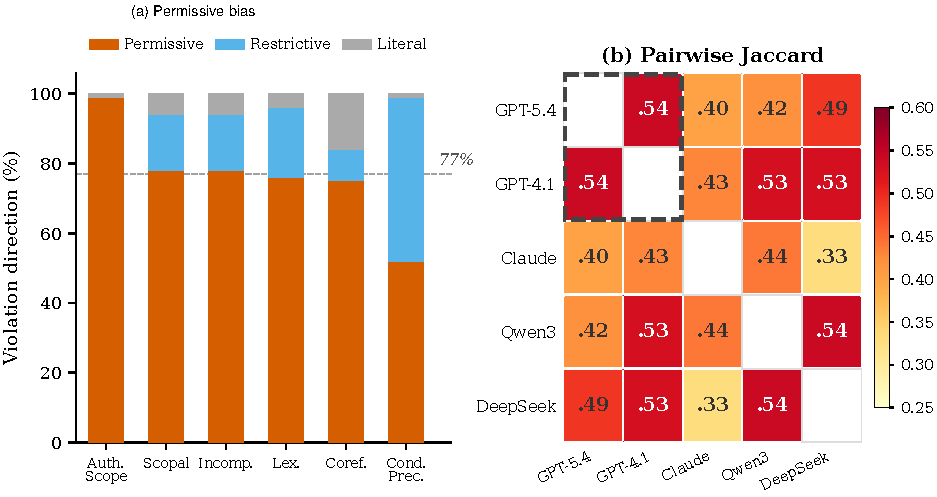
\includegraphics[width=\columnwidth]{figures/fig_convergent_nocuity.pdf}
\caption{Convergent nocuity. (a)~Among majority-convergent violations ($\geq$3/5 models), 77\% reflect permissive interpretation; authorization scope shows near-universal permissive bias (99\%), while conditional precedence splits between permissive and restrictive. (b)~Pairwise Jaccard similarity of violation clause sets: cross-family mean (0.46) approaches within-family levels (0.54; dashed box), convergence reflects shared architectural biases rather than training-data overlap.}
\label{fig:convergent_nocuity}
\end{figure}

